% !TeX program = xelatex
\documentclass{beamer}
\usepackage{ctex}
\usepackage{hyperref}
\usepackage{soul}

\title{Hacking Git - a Blocktree}
\author{陈嘉杰}
\date{2018 年 10 月}

\begin{document}
\begin{frame}
    \maketitle
\end{frame}

\begin{frame}{Git 是个{\bf 啥子}}
    大家知道 Git 是什么吗?
    
    \includegraphics<1->[width=\linewidth]{2018-10-25-08-44-33.png}

    \pause
    the stupid content tracker

    \pause
    a block tree
\end{frame}

\begin{frame}{先开始动手}
    咱们边做边讲,先请大家安装一下 Git :

    \$ apt install -y git

    \pause

    然后设置一下自己的名字和邮箱:

    \$ git config -{}-global user.name "Jiajie Chen"

    \$ git config -{}-global user.email "jiegec@qq.com"

    \pause

    然后新建一个文件夹,在里面建立一个空的 Git 仓库:

    \$ mkdir learn\_git

    \$ cd learn\_git

    \$ git init

\end{frame}

\begin{frame}{Git 能做什么}
    Git 是一个 “版本控制系统” ,这意味着:

    \begin{itemize}
        \item 保存你文件修改的历史记录,你可以看到你以前在什么时候都做了什么更改
        \item 可以多人同时工作在同一个项目里,合理地把大家写的代码合并
        \item 学好了 Git ,有利于软工等课程的学习
        \item 学会了 Git ,你就可以参与到 GitHub 的广阔开发者社区中
        \item 学会了 Git ,你才能有朝一日成为 Linux Kernel 开发者
    \end{itemize}

    不要怕,让我们一点一点来。最后自然也有给大家的一个挑战环节。
\end{frame}

\begin{frame}[fragile]{保存文件历史记录}
    假如要记录和妹子的出游记录(基于 NanoApe 真实事件改编)

    \$ echo "2018-10-04 Shenyang" >{}> log.txt

    \$ git status
    
    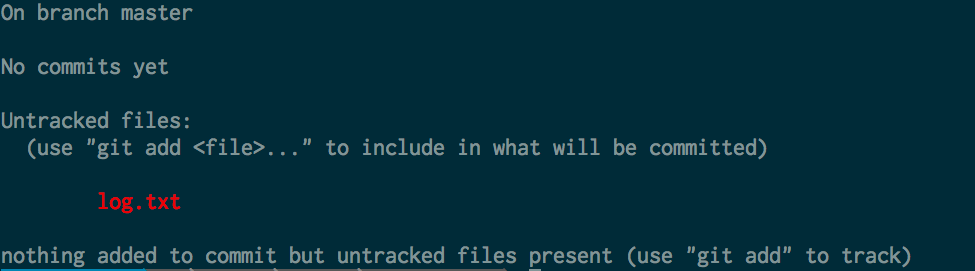
\includegraphics[width=\linewidth]{2018-10-25-09-30-24.png}
\end{frame}

\begin{frame}{git add}
    Git 默认情况下不会把你的文件考虑进来。你必须告诉 Git 让它替你管理这个文件的历史记录。我们采用的命令是:

    \$ git add log.txt

    当然了,它还有别的写法,我们经常会用

    \$ git add .

    来把当前目录和所有子目录里文件都加进来。小提示:你可以试试 git add -i 的效果。执行以后,是这个效果:
    
    \$ git status

    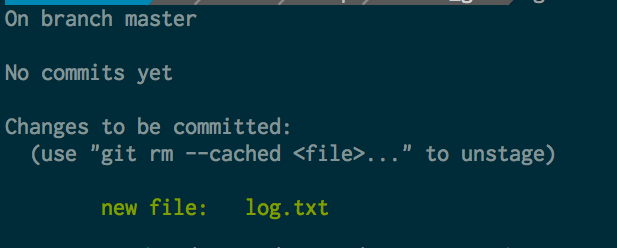
\includegraphics[width=\linewidth]{2018-10-25-09-33-45.png}

\end{frame}

\begin{frame}{年轻人的第一个提交!}
    Git 有暂存区(stage)的概念,允许你在最终决定一个版本前先做一些修改。git add 把当前文件系统的更改添加到暂存区,而 git commit 则把暂存区的更改保存在历史记录中。

    首先我们可以看看暂存区有什么内容:

    \$ git diff --cached
    
    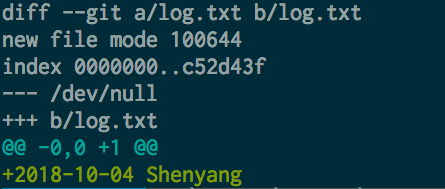
\includegraphics[width=\linewidth]{2018-10-25-09-49-00.png}

    这个格式叫做 Unified Diff 。以后大家还会经常看到。
\end{frame}

\begin{frame}{年轻人的第一个提交!(续)}
    然后 NanoApe 检查了一下,时间和地点都没错,保存!

    \$git commit -m "Add shenyang tour"

    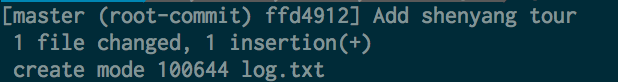
\includegraphics[width=\linewidth]{2018-10-25-09-55-12.png}

    我们再看一下当前的状态:

    \$ git status

    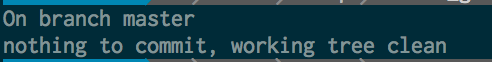
\includegraphics[width=\linewidth]{2018-10-25-09-55-36.png}

    妙啊,我的文件都已经保存进去了。那我想看我之前都做了什么,怎么办?
\end{frame}

\begin{frame}{git log}
    有一个命令可以查看最近的提交: git log

    \$ git log
    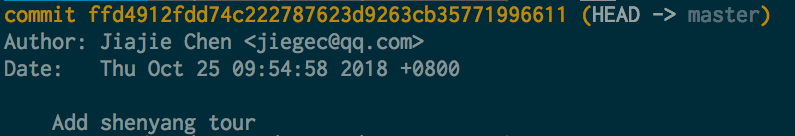
\includegraphics[width=\linewidth]{2018-10-25-09-59-01.png}

    可以看到我在这个时候添加了一个提交,作者是我,时间是这个时间,然后这个提交的描述是这个。

\end{frame}
\begin{frame}{git log (续)}
    怎么看这个提交具体做了什么呢?

    \$ git log -p

    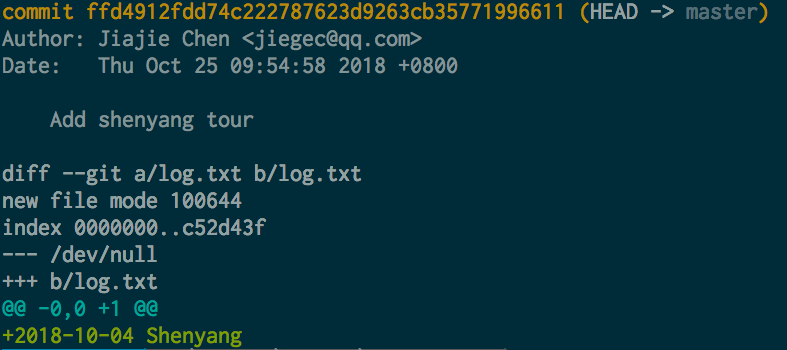
\includegraphics[width=\linewidth]{2018-10-25-10-01-41.png}

    它还支持很多写法,比如 HEAD\^{}\^{}..HEAD 表示从显示当前提交往前走两个,从它开始到当前提交的历史记录。
\end{frame}

\begin{frame}{一个提交太单调,我们加多一个}
    \$ echo "2018-10-24 128 Days" >{}> log.txt

    \$ git commit -a -m "Add 1024 day"

    \$ git log -p

    注: git commit -a -m "abc" 相当于 git add . \&\& git commit -m "abc"

\end{frame}

\begin{frame}
    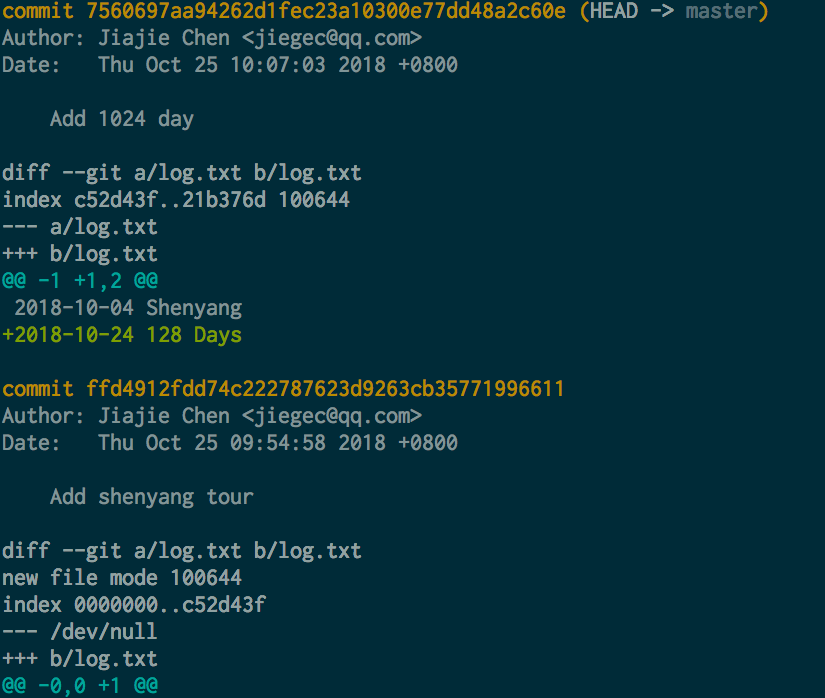
\includegraphics[width=\linewidth]{2018-10-25-10-46-39.png}
\end{frame}

\begin{frame}{啊,忘了一件事情}
    NanoApe: 唔,忘记提妹子的 ID 了,这不行。我得改一下

    \$ cat log.txt

    2018-10-04 Shenyang

    2018-10-24 128 Days with muvseea

    \$ git status

    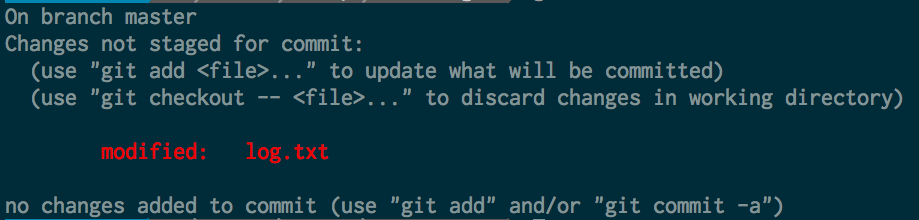
\includegraphics[width=\linewidth]{2018-10-25-10-49-26.png}
\end{frame}

\begin{frame}{啊,忘了一件事情(续)}
    我们可以看到刚刚的更改:

    \$ git diff

    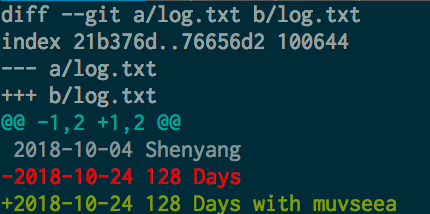
\includegraphics[width=\linewidth]{2018-10-25-10-50-20.png}
\end{frame}

\begin{frame}{啊,忘了一件事情(续续)}
    我看刚才的提交不爽,可不可以更改我上一次的提交?可以:

    \$ git commit -a -{}-amend -m "Add 128 days with muvseea"

    \$ git log

    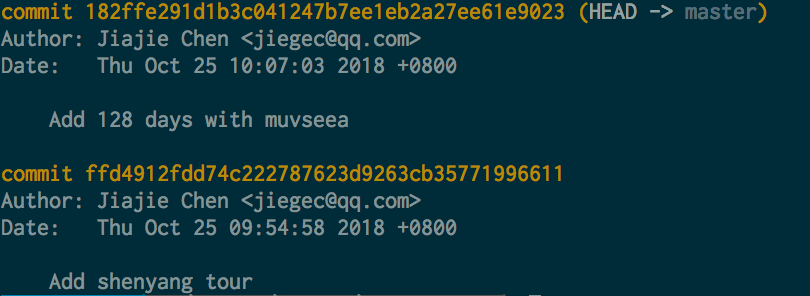
\includegraphics[width=\linewidth]{2018-10-25-10-52-16.png}
\end{frame}

\begin{frame}{谈谈暂存区}
    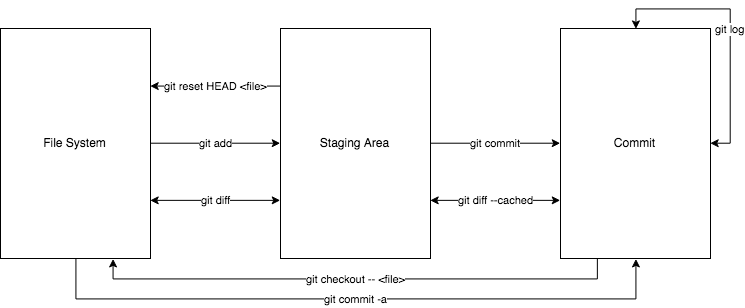
\includegraphics[width=\linewidth]{2018-10-25-11-01-32.png}

    "git status" is your firend.
\end{frame}

\begin{frame}{Pro Git 上的类似表述}
    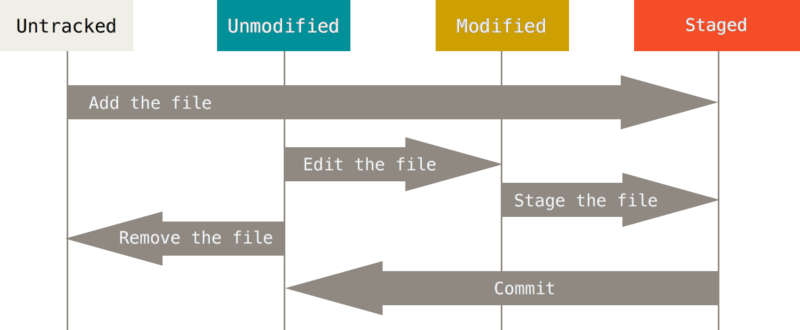
\includegraphics[width=\linewidth]{lifecycle.png}
\end{frame}

\begin{frame}{发布虐狗版本!}
    \$ git tag nue-gou-1.0

    \$ git log

    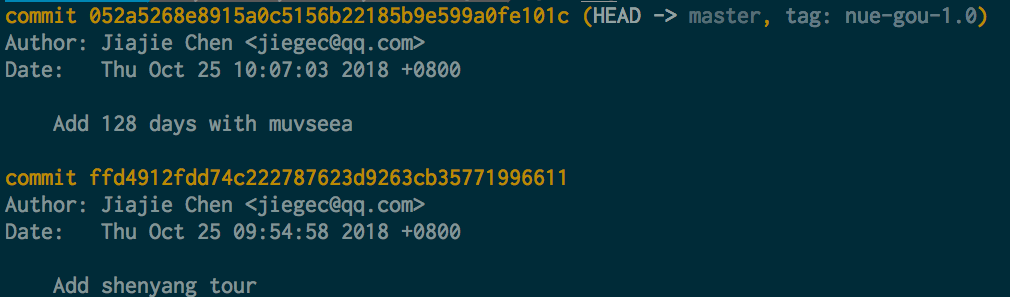
\includegraphics[width=\linewidth]{2018-10-25-11-16-26.png}

    这样我们就创建了一个名为 nue-gou-1.0 的 tag 。查看所有的 tag :

    \$ git tag

    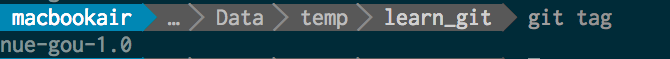
\includegraphics[width=\linewidth]{2018-10-25-11-18-36.png}
\end{frame}

\begin{frame}{虐狗回顾}
    假如 NanoApe 虐狗了 99 年的时候,想看一下当年的自己?(好浪漫啊)

    \$ git checkout nue-gou-1.0

    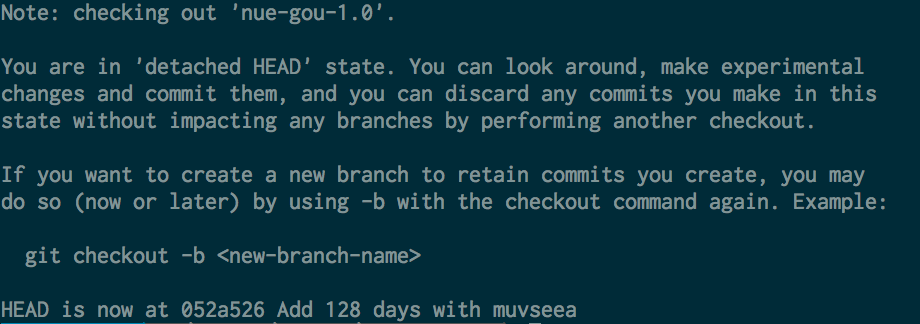
\includegraphics[width=\linewidth]{2018-10-25-11-21-49.png}

    这样就可以回到当时的这个版本。实际上就是对某个 commit 进行了命名。

    \$ git checkout master

    恢复到原来的地方
\end{frame}

\begin{frame}{Git 协作}
    经过上面这部分,你应该已经学会如何用 Git 管理自己的代码了。但 Git 的强大很大程度在于,可以让很多人一起在一个项目上工作。

    我们以清华 Git 为例。

    \url{https://git.tsinghua.edu.cn}

    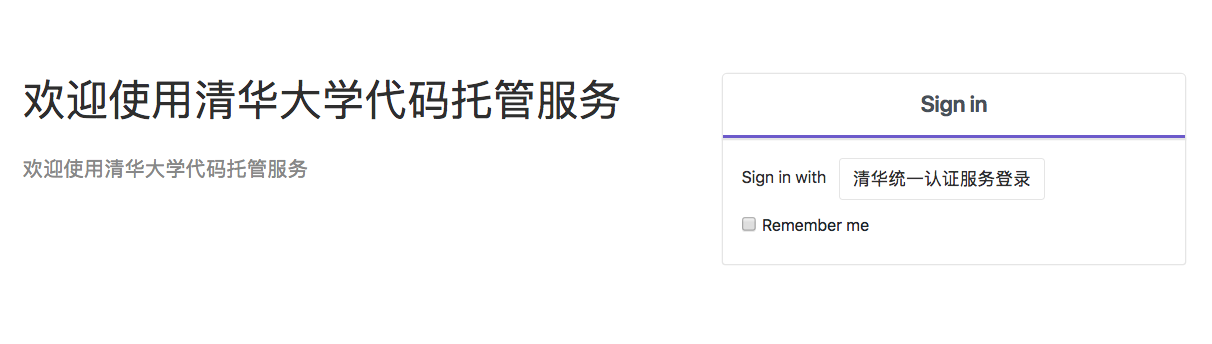
\includegraphics[width=\linewidth]{2018-10-25-11-31-40.png}

    使用清华 ID 登录即可。
\end{frame}

\begin{frame}{GitLab 配置}
    进去后,点击右上角的图标,点击 Settings

    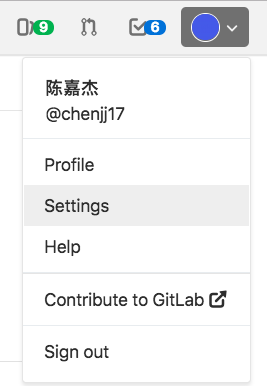
\includegraphics[width=0.5\linewidth]{2018-10-25-11-37-23.png}
\end{frame}

\begin{frame}{GitLab 配置(续)}
    在左下角找到 SSH Keys

    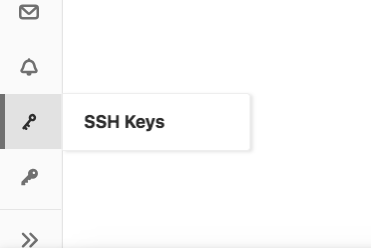
\includegraphics[width=\linewidth]{2018-10-25-11-38-45.png}
\end{frame}

\begin{frame}{GitLab 配置(续续)}
    如果大家还没有生成过,回到终端,生成一个自己的 SSH Key :

    \$ ssh-keygen

    按照要求生成 SSH Key 。注意保存!拥有这个 Key 就可以对你拥有的 GitLab 仓库进行修改。

    然后查看 \~{}/.ssh/id\_rsa.pub 文件的内容,复制到浏览器中,输入一个名称,最后添加到 GitLab 中。效果如图:

    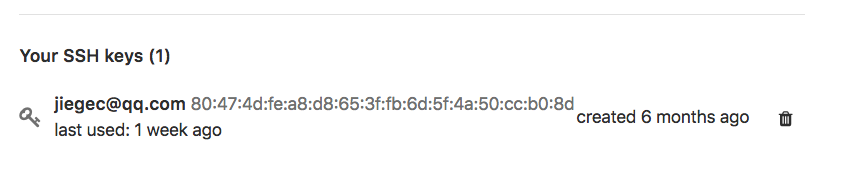
\includegraphics[width=\linewidth]{2018-10-25-11-42-06.png}

    测试一下是否成功配置了:

    \$ ssh -T git@git.tsinghua.edu.cn

    应该会输出 Welcome To GitLab 的信息。

\end{frame}

\begin{frame}{创建仓库}
    找到 New Project ,进入创建仓库界面 \url{https://git.tsinghua.edu.cn/projects/new}

    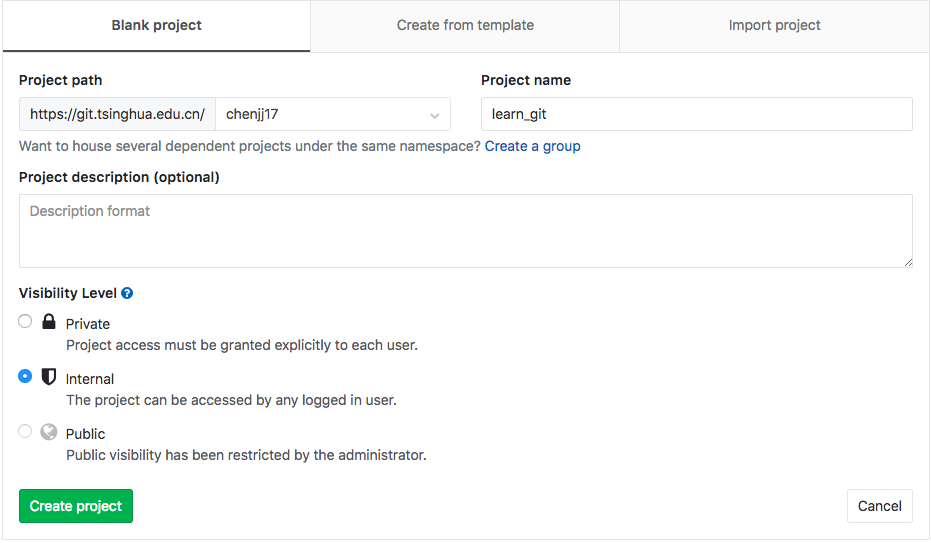
\includegraphics[width=\linewidth]{2018-10-25-11-54-08.png}

    点击 Create Project 。

\end{frame}

\begin{frame}{把刚才的仓库推到 GitLab 上}
    \$ git remote add origin git@git.tsinghua.edu.cn:chenjj17/learn\_git.git
    
    \$ git push origin master

    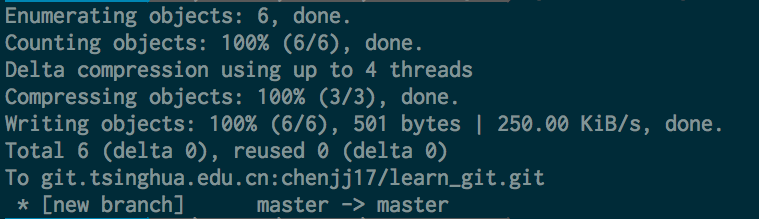
\includegraphics[width=\linewidth]{2018-10-25-11-59-01.png}

    这时候就能在 GitLab 上看到我们刚才提交的更改

    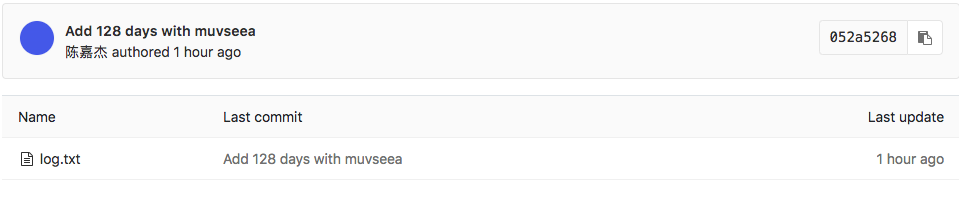
\includegraphics[width=\linewidth]{2018-10-25-12-02-10.png}
\end{frame}

\begin{frame}{多人同时在不同分支协作}
    这次请出我们的两位主人公,muvseea 和 NanoApe 来给他们的虐狗日记添加一些内容。。。

    NanoApe:

    \$ git checkout -b nanoape

    \$ ...

    \$ git commit -m "Add credit"

    \$ git push origin nanoape

    muvseea:

    \$ git checkout -b muvseea

    \$ ...

    \$ git commit -m "Add new log and edit an old one"

    \$ git push origin muvseea
\end{frame}

\begin{frame}{协作!}
    这时候可以看到,两人都对虐狗日记添加了自己的更改:

    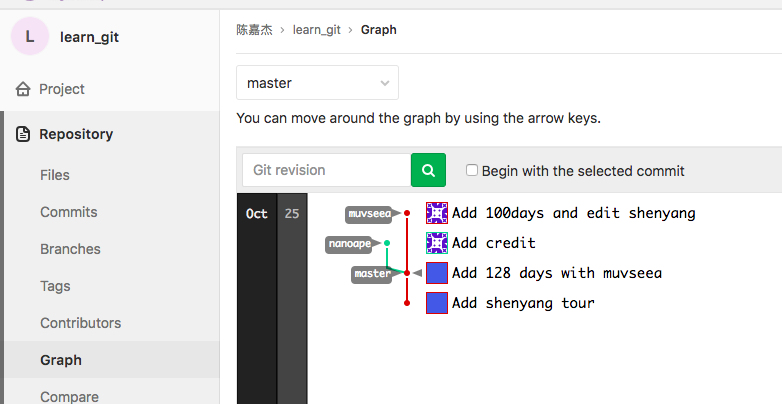
\includegraphics[width=\linewidth]{2018-10-25-13-09-01.png}
\end{frame}

\begin{frame}{合并?}
    现在 NanoApe 和 muvseea 都对自己更新很满意了,想要把各自的更新合并回 master 分支里。那么,NanoApe 此时应该打开一个 Merge Request :

    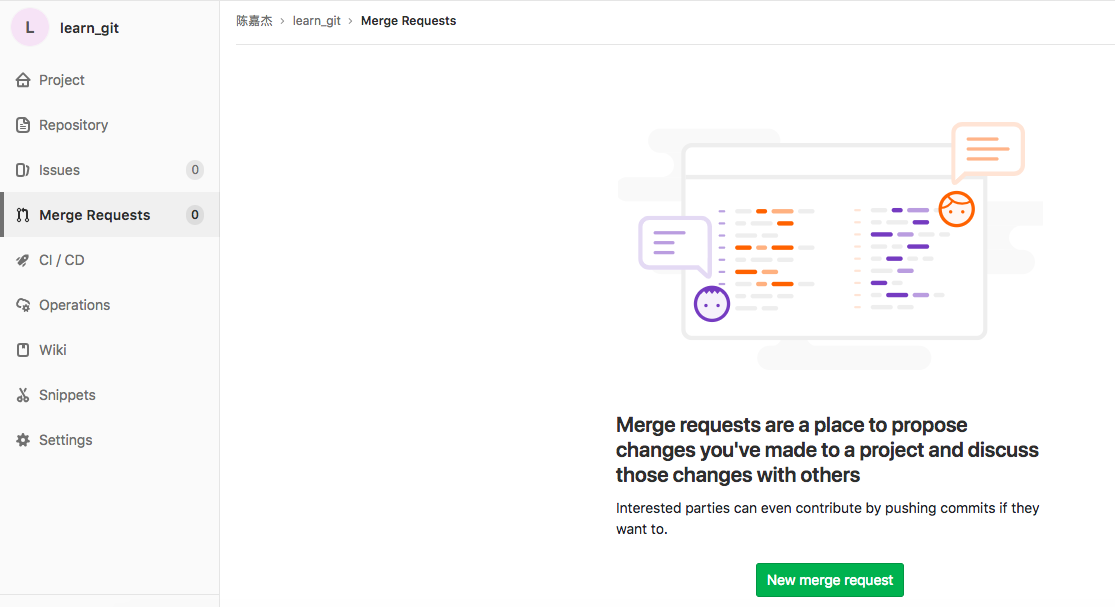
\includegraphics[width=\linewidth]{2018-10-25-16-49-36.png}
\end{frame}

\begin{frame}{合并?(续)}
    指定要从 nanoape 分支合并入 master 分支:

    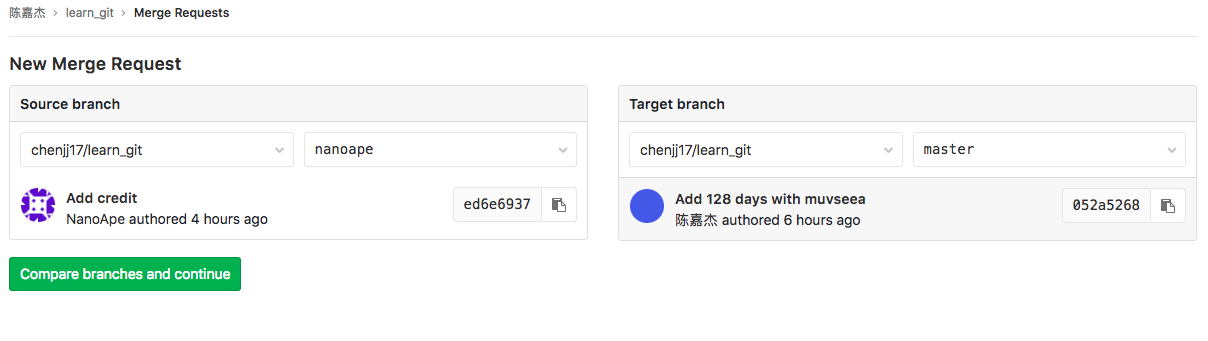
\includegraphics[width=\linewidth]{2018-10-25-16-50-58.png}

    点击 Compare branches and continue , 然后找到下面的 Submit merge request ,这就创建了一个 Merge Request :

    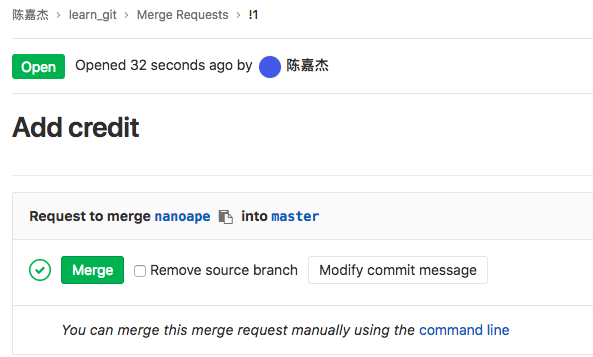
\includegraphics[width=\linewidth]{2018-10-25-16-52-33.png}
\end{frame}

\begin{frame}{合并!}
    点击 Merge ,这时候看一下提交历史:

    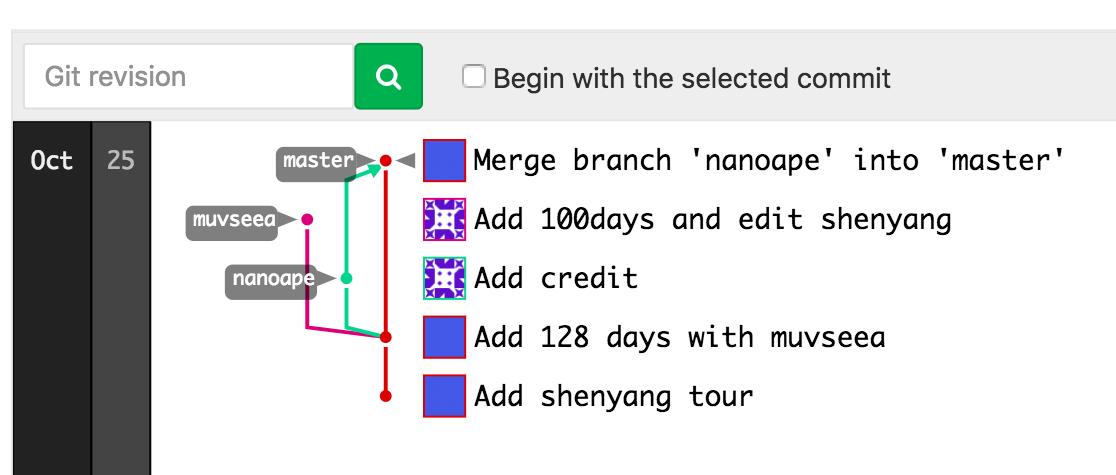
\includegraphics[width=\linewidth]{2018-10-25-16-54-11.png}

    查看此时 master 分支上的 log.txt ,发现已经有了 NanoApe 进行的更改。

    接下来,我们让 muvseea 也来一次同样的操作。
\end{frame}

\begin{frame}{冲突?}
    我刻意创造了一个情况,就是 NanoApe 和 muvseea 对同一行内容进行了修改。此时在 muvseea 创建 Merge Requests 的时候,就需要首先 Resolve Conflict:

    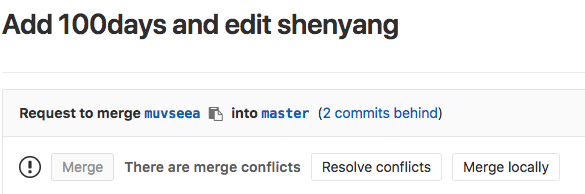
\includegraphics[width=\linewidth]{2018-10-25-16-56-59.png}
\end{frame}

\begin{frame}{别吵架了!}
    点击 Resolve conflicts ,我们可以看到是哪里冲突了

    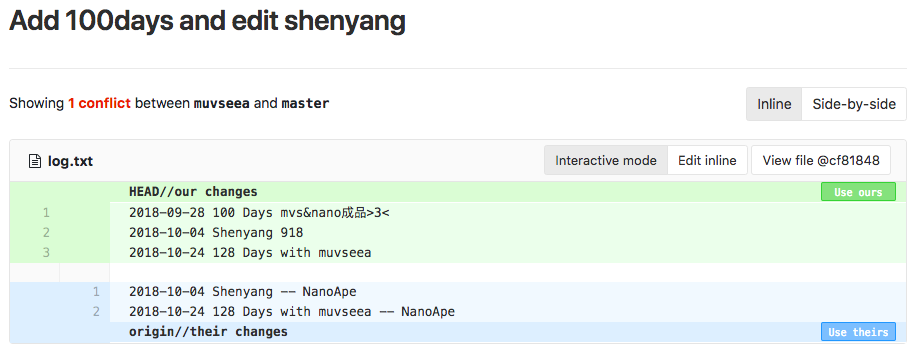
\includegraphics[width=\linewidth]{2018-10-25-16-57-53.png}

    上面是 muvseea 做的更改,下面是 NanoApe 做的更改。这里我们可以选择采用 muvseea 修改的版本,也可以选择采用 NanoApe 修改的版本,也可以选择 Edit inline 自己进行冲突的合并。

    手动更改后,点击下面的 Commit 把冲突解决,然后点击 Merge 把修改合并到 master 分支。
\end{frame}

\begin{frame}{等等\ldots 发生了什么?}
    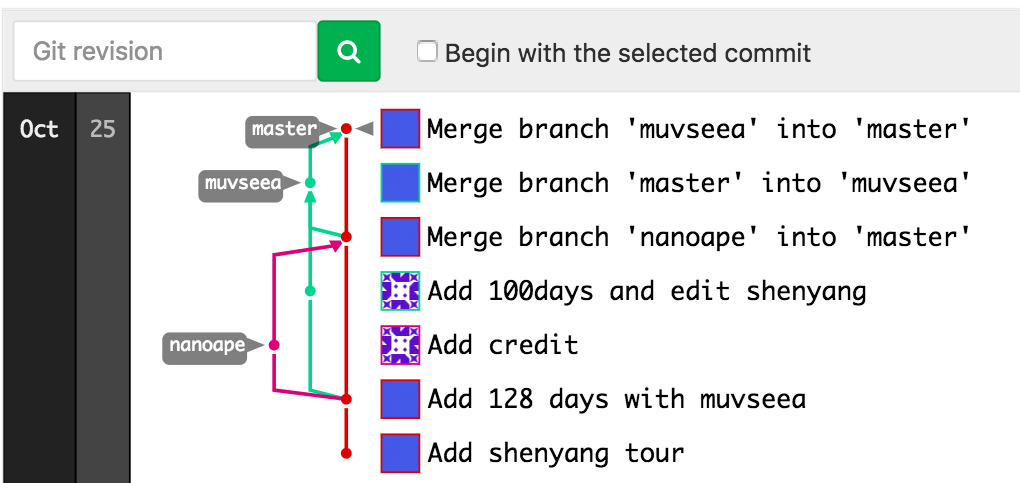
\includegraphics[width=\linewidth]{2018-10-25-17-01-54.png}
    现在,NanoApe 和 muvseea 做的更改都合并到了 master 分支中。双方的更改都可以看到。
\end{frame}

\begin{frame}{本地和 Gitlab 同步}
    刚才我们的操作都在 Gitlab 上进行。如何在本地获取到我们在网页上合并的结果呢?

    \$ git fetch

    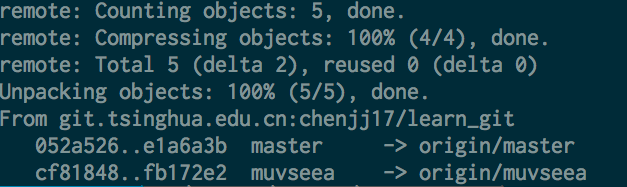
\includegraphics[width=\linewidth]{2018-10-26-19-25-28.png}
\end{frame}

\begin{frame}{本地和 Gitlab 同步}
    此时的提交历史:

    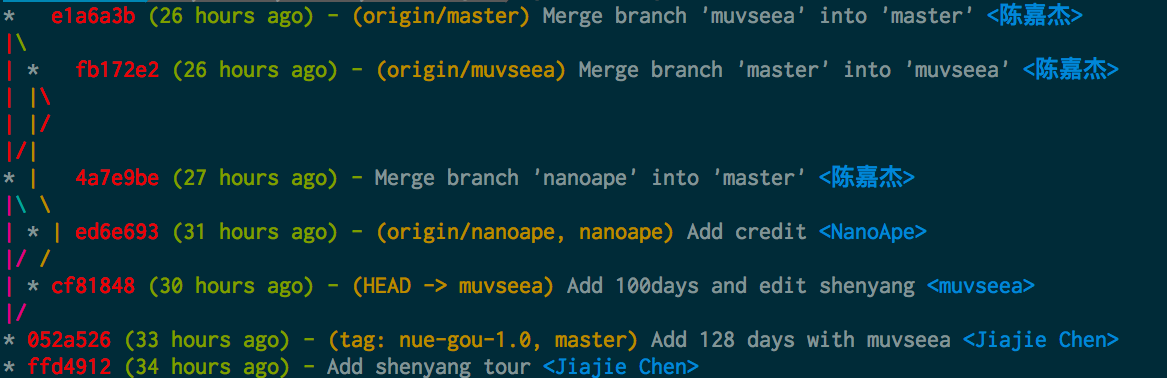
\includegraphics[width=\linewidth]{2018-10-26-19-27-09.png}
    
    注意,这里的 origin 代表我们之前添加的 remote ,即 Gitlab 。 这里的 origin/master 代表 Gitlab 上的 master 分支,它现在所在的位置和本地的 master 分支不同。
\end{frame}

\begin{frame}{本地和 Gitlab 同步(续)}
    当然了,我们更常用的命令是:

    \$ git pull origin master

    它不仅会拉取当前上游的提交,而且会把本地的 master 分支更新到上游的版本。

    不过,有时候,我们在本地更改了一些内容的时候,这个命令会报错:因为你进行了修改,不允许你直接更新到上游的版本。这时候我们可以这样:

    \$ git stash

    它会把当前的更改保存为一个临时的 commit 并且回退到之前的状态。之后当你想回到这个修改后的状态的时候,你可以:

    \$ git stash apply

    它会尝试把你的更改应用过来,不过并不会删掉这个临时的 commit 。你也可以选择
    
    \$ git stash pop

    来应用并在成功的时候删除掉它。如果要删掉全部的临时 commit ,你也可以:

    \$ git stash clear
\end{frame}

\begin{frame}{Recap}
    我们想想,如果我们要合并两个人做的事情,应该怎么做?

    举个栗子:

    \begin{enumerate}
        \item 有个图书馆,一开始没有书,经过了若干天后,有 3 本书
        \item 第一个人看中了一本书,想,今晚我要这本书。
        \item 第二个人想还一本书,想,今晚我把这本书还到这里。
        \item 到了晚上,图书管理员和这两个人见面了。他看了下第一个人要借书,嗯,拿去。第二个人要还书,嗯,放下。这时候是 3 - 1 + 1 本书。
        \item 他记下:书[0] A 借了;书[3] B 还了。
    \end{enumerate}

    这实际上是三个状态的合并:原来的 3 本书;第一个人取走书后的 2 本书;第二个人还了书的 4 本书。
\end{frame}

\begin{frame}{Conflict?}
    那在什么情况下可能出现冲突呢?

    还是这个栗子:

    \begin{enumerate}
        \item 有个图书馆,一开始没有书,经过了若干天后,有 3 本书
        \item 第一个人看中了一本书,想,今晚我要这本书。
        \item 第二个人也看中了这本书,想,今晚我要这本书。
        \item 到了晚上,图书管理员和这两个人见面了。他看了下第一个人和第二个人要借的书一样,唔,行,那我借出去了,但是给谁,你们自己打一架决定。
    \end{enumerate}

    所以冲突的产生在于:不同人对同一个东西做了不同的更改。
\end{frame}

\begin{frame}{Git 的智能合并策略}
    从上面这个栗子我们可以看到,一些时候我们是可以很好地合并两个人的更改的。

    而这个更改,实际上就是,从两人的提交的最近的共同祖先到这两个提交的改变。

    通过把只有一方改变的地方合并起来,把双方都改变的地方要求用户去解决,这就是三路合并。

    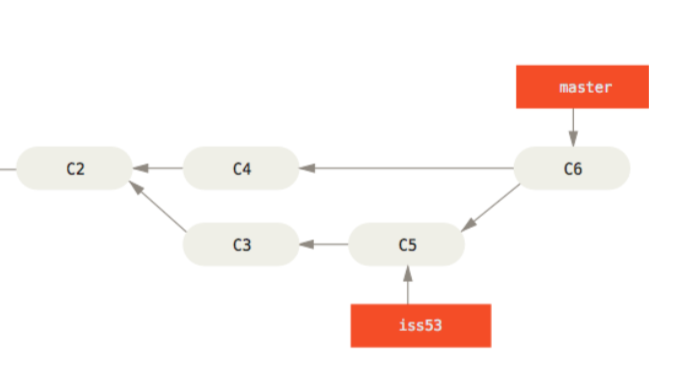
\includegraphics[width=\linewidth]{2018-10-26-16-15-08.png}
\end{frame}

\begin{frame}{分支!?}
    刚才还提到了一个东西:分支。

    分支实际上就是一个一直跟随 commit 在变的标记。

    比如 master 分支,它代表着项目代码当前最新的一个提交。而 nanoape 分支,则代表 NanoApe 对代码更改的最新的一个提交。

    实际上在合并的时候可以直接指定和哪个提交进行合并。

    在真实的项目中,我们往往会进一步细分: develop 表示正在活跃开发的版本, release 表示已经发布的最新版本,等等。
\end{frame}

\begin{frame}{分支的常见操作}
    创建一个新分支,它指向的 commit 为当前 commit

    \$ git branch [name]

    切换到指定的分支

    \$ git checkout [name]

    创建并切换到分支

    \$ git checkout -b [name]

    显示所有的分支

    \$ git branch

    删除分支

    \$ git branch -d [name]
\end{frame}


\begin{frame}{合并的骚操作??}
    不过,合并当然不仅有三路合并这一种方法。大家还有很多骚操作的,比如:

    \begin{itemize}
        \item 变\quad 基(rebase)。意思就是在新的上游上重放你的更改。当然了,一样会有冲突的问题,但是最后的提交历史会是一条直线。变基可以用的很复杂,我就不深入讲了,太黑科技了。
        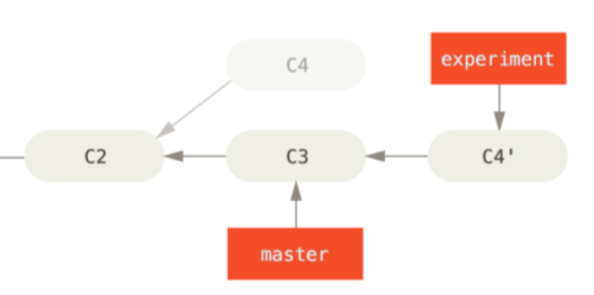
\includegraphics[width=\linewidth]{2018-10-26-16-23-42.png}
        \item Squash ,就是把你的更改全部合并成一个提交,再合并进去。
    \end{itemize}
\end{frame}

\begin{frame}{热热热}
    烫烫烫热热热rerere

    git 有个不为人知的功能,叫 Rerere (Reuse recorded resolution)。它会记录你解决冲突的历史记录,然后当你下次遇到同样的冲突的时候,它会自动帮你解决。

    \$ git config -{}-global rerere.enabled true

    即可开启。免费的人工智能!
\end{frame}

\begin{frame}{讲一些奇怪的操作}
    如果你要魔改提交历史的话:

    \$ git rebase [commit]

    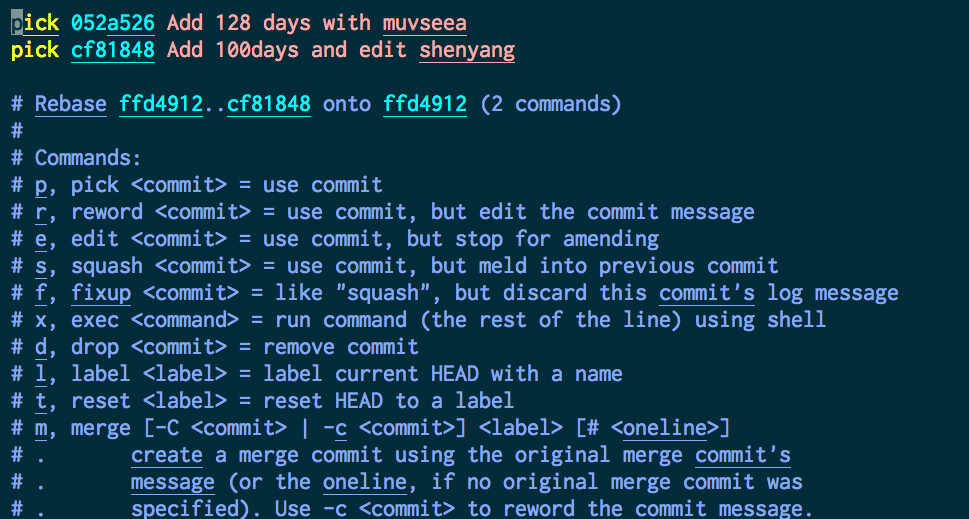
\includegraphics[width=\linewidth]{2018-10-26-20-03-30.png}

    魔改完可以用 \$ git push -{}-force 强制提交到上游

    注意,Gitlab 默认禁用了 master 分支的强制 push 。如非必要,请勿打开这个开关。
\end{frame}

\begin{frame}{如果你不小心把密码存在了仓库里并且传给了别人}
    可以一条命令把一段历史中某个文件都删掉:

    \$ git filter-branch -{}-tree-filter 'rm -f password.txt' HEAD

    魔改完可以用 \$ git push -{}-force 强制提交到上游

    然后还是建议赶紧改密码。

    还可以批量把提交者的名字改了:

    \$ git filter-branch -{}-commit-filter 'GIT\_AUTHOR\_NAME="Linus Torvalds" GIT\_AUTHOR\_EMAIL="torvalds@linux-foundation.org" git commit-tree "\$@"'

    这样你就可以伪装成 Linus Torvalds 提交代码了。

    当然了,如果不是密码这么敏感的信息,你可以用

    \$ git revert [commit]

    生成一个效果和某个 commit 抵消的 commit。
\end{frame}

\begin{frame}{如何保证以我的名字提交的就是我提交的?}
    需要大家配一下自己的 GPG Key ,过程比较复杂,这里就不详细讲了。

    配好后,在提交的时候这么写:

    \$ git commit -S -m [message]

    然后在网页上就会这么显示:

    
\includegraphics[width=\linewidth]{2018-10-26-20-16-02.png}

    这个基于的是 GPG Key 的信任模型,大家有兴趣的话可以了解一下。
\end{frame}

\begin{frame}{嘿,接锅嘞}
    突然有一天,代码出了 BUG ,发现是一个很愚蠢的地方写错了。你想知道这行代码是谁改的,然后劈头盖脸骂ta一顿。怎么看?

    \$ git blame [file]

    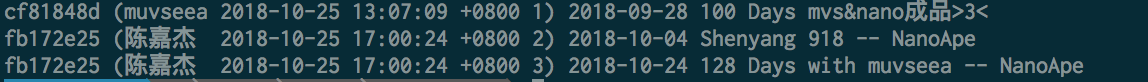
\includegraphics[width=\linewidth]{2018-10-27-00-12-08.png}

    可以看到每一行最后都是谁改的,什么时候改的,这些内容。
\end{frame}

\begin{frame}{嘿,接锅锅嘞}
    再设想一种情况:你看了看代码,不知道哪里有问题,但你知道啥时候肯定是好的。那我们自然会想,能不能二分呢?可以:

    \$ git bisect start

    \$ git bisect bad

    这样,标记了当前的 commit 是坏的。然后,再标记一个没有问题的 commit :

    \$ git bisect good [commit]

    之后,它会自动选择好和坏中央的 commit ,你测试一下代码是否工作然后根据好坏继续执行:

    \$ git bisect good/bad

    最后就可以定位到出错的地方了。
\end{frame}

\begin{frame}{Block\st{chain}tree}
    Git 里每个 commit 都有一个很长的十六进制值:它目前是这些内容的 SHA-1 (以后会换哈希算法)

    \begin{itemize}
        \item 提交的信息
        \item 提交人
        \item 提交日期
        \item 作者
        \item 编辑日期
        \item 整个目录树结构的哈希值
    \end{itemize}
\end{frame}

\begin{frame}{举个栗子}
    \$ git rev-parse HEAD | xargs git cat-file -p

    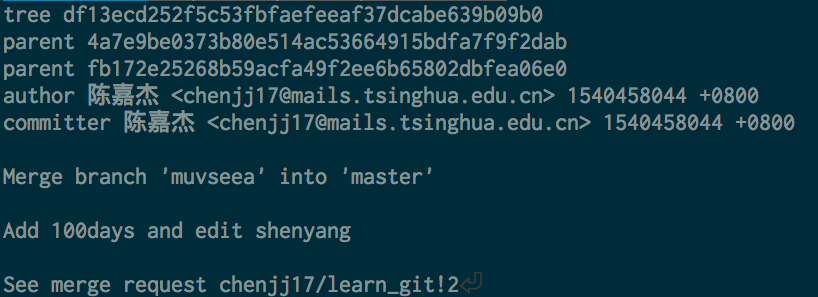
\includegraphics[width=\linewidth]{2018-10-26-21-50-58.png}
\end{frame}

\begin{frame}{目录结构是个什么?}
    \$ git cat-file -p df13ecd252f5c53fbfaefeeaf37dcabe639b09b0 

    
\includegraphics[width=\linewidth]{2018-10-26-21-54-08.png}

    \$ git cat-file -p beea1aa47abadc02495171084f5afdc4f4eb4ade

    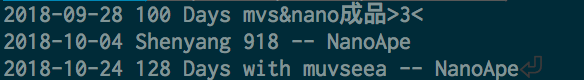
\includegraphics[width=\linewidth]{2018-10-26-21-55-01.png}
\end{frame}

\begin{frame}{看个图}
    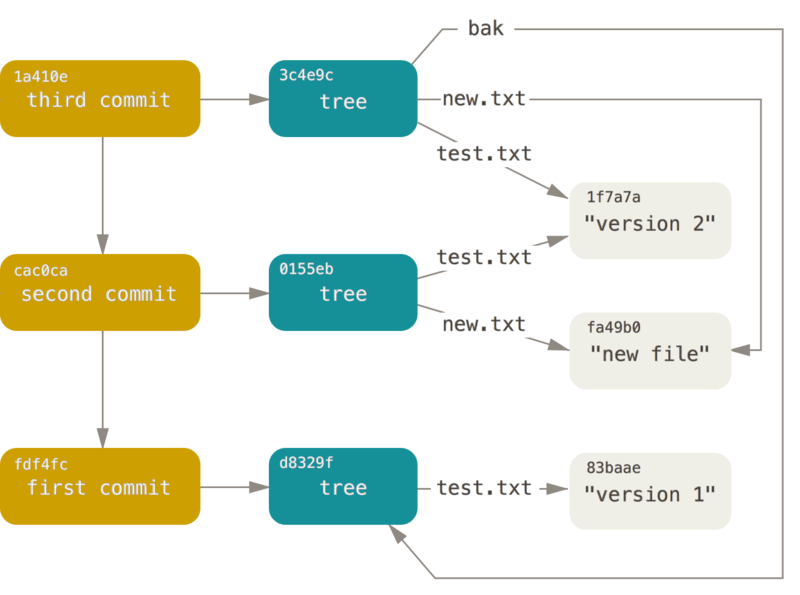
\includegraphics[width=\linewidth]{2018-10-26-21-48-43.png}
\end{frame}

\begin{frame}{如何手动创建一个 commit ?}
    把文件保存到 Git 中,得到它的哈希值

    \$ git hash-object -w [file]

    把该文件添加到暂存区

    \$ git update-index -{}-add -{}-cacheinfo 100644 [file\_hash] [file]

    生成当前目录树的哈希

    \$ git write-tree

    生成提交的哈希

    \$ echo 'commit message' | git commit-tree [tree\_hash] -p [parent\_hash]

    把当前的 master 分支指向刚刚创建的提交

    \$ git update-ref refs/heads/master [commit\_hash]
\end{frame}

\begin{frame}{查看 HEAD 的历史}
    我们知道 HEAD 是一个特殊的“指针”,一直指向目前的提交。

    而我们常常会不小心把某个 commit 弄丢。也就是说,它不在现在的任何一个分支上。这咋办呢?

    \$ git reflog

    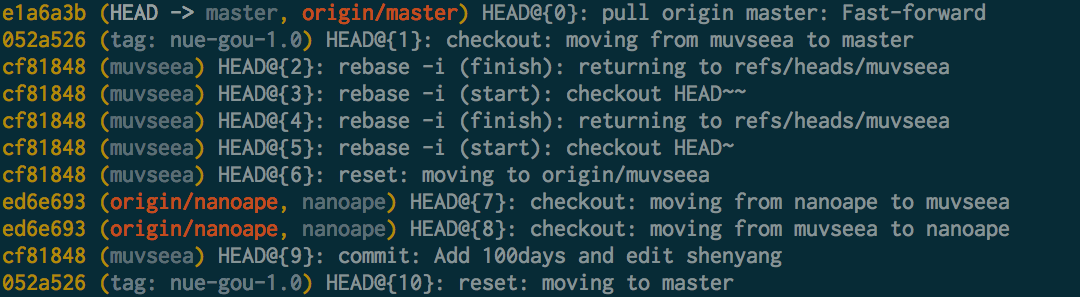
\includegraphics[width=\linewidth]{2018-10-26-23-23-26.png}

    它会记录你的 HEAD 变更历史。这样,即便你不小心弄丢了什么,还有很大机会可以找回来。

    当然了,你也可以用

    \$ git fsck -{}-full

    它会找到所有的悬孤提交(dangling commit),也是一样的效果。
\end{frame}

\begin{frame}{什么时候孤儿 commit 历史会丢呢?}
    有个命令,会在你的图上跑个搜索,标记上各个分支可以连接到的 commit ,然后把没有标记到的文件删除。

    \$ git gc

    也就是垃圾回收。同时,为了节省空间,它会把很多个小文件打包成一个大的压缩包,并把一些文件用 diff 的形式保存下来。这在很大的仓库里会非常有用。
\end{frame}

\begin{frame}{Git 的本质是。。。?}
    复读机(误

    区块树+Key-Value存储

    每个数据的 Key 是它本身的 SHA-1 哈希值,Value 就是文件本身的内容。

    区块树:每个提交记录了它的父提交的 SHA-1 值。在 SHA-1 不能任意制造碰撞前,可以保证这是一棵树,并且确定了一个 commit 的 SHA-1 几乎无法伪造一个假的历史。
\end{frame}

\begin{frame}{最新研究:Git 可以打环辣}
    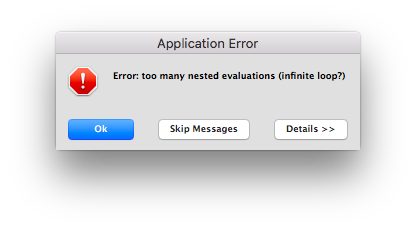
\includegraphics[width=\linewidth]{2018-10-26-23-52-53.png}
\end{frame}

\begin{frame}{dbq 假新闻}
    采用了一个命令:

    \$ git replace

    它能做到,把一个 commit 替换成另一个 commit 。一个用途是可以拆分历史后再合并两个历史。

    实际上并没有修改这颗区块树,只是人为假装修改了一些边而已。

    实测, GitHub 和 GitLab 的绘制 Commit Graph 的工具会直接忽略这个。而 git log -{}-graph 检测到打环后直接就停在中间不输出了。

    不过, Gitk 就没有这么好运气了。它大概是没人维护了,于是就,无限循环了。
\end{frame}

\begin{frame}{喜闻乐见的 Bonus 环节}
    \$ git clone git@git.tsinghua.edu.cn:chenjj17/hacking\_git.git

    在仓库里,有一个名为 learn\_git.tar.gz 的文件。这样解压:

    \$ tar xvf learn\_git.tar.gz

    你会看到有一个名为 learn\_git 的目录解压出来。进去以后,这是一个 Git 仓库,里面藏了一个红包。

    提示:回忆一下我刚才讲到的一些命令,我会把东西隐藏到哪儿呢?
\end{frame}

\begin{frame}{没有讲到的但可能会用到的}
    \begin{itemize}
        \item diff 和 apply
        \item textconv 过滤器
        \item ident 和 filter
        \item hooks 和 CI
        \item svn 集成
        \item 如何用邮件和别人协作
    \end{itemize}

    扩展阅读:墙裂推荐 《Pro Git 2》 网上有开源版本可以自己构建、阅读。
\end{frame}

\end{document}
